% !TeX root = sigqdyn_tr.tex
% ================================================================
\section{The Time to Measure the Service Time of a Queue}\label{sec:svc_time}

In around 2012, it became recognized that one of the main problems with AQMs was the sensitivy of their configuration to changing environments. For example:
\begin{itemize}
	\item access links often change their rate when modems retrain in response to interference. 
	\item a queue can be part of a scheduling hierarchy and traffic in higher priority queues varies the capacity left for a lower priority queue, rapidly varying the drain rate that the AQM experiences.
	\item the capacity of radio links varies rapidly over time~\cite{McGregor10:Minstrel_TR}.
\end{itemize}

The CoDel algorithm~\cite{Nichols12:CoDel} proposed to solve this problem by measuring the queue in units of time, rather than bytes. This made the configuration of the thresholds in the algoithm independent of the drain rate.

Actually, as far back as 2002, 
Kwon and Fahmy~\cite{Kwon02:Load_v_Queue_AQM} had advised that the queue should 
be measured in units of time. Also, in 2003, S{\aa}gfors \emph{et al} had 
modified the Packet Discard Prevention Counter (PDPC+~\cite{Sagfors03:PDPC_vary}) 
algorithm by converting queue length to queuing delay to cope with the varying 
link rate of 3G wireless networks.

PDCP still measured the queue in bytes, but then converted the result to time by dividing by the link rate, which it measured over a brief interval. 

CoDel proposed an elegant way to measure the service time of the queue by adding a timestamp to each packet's internal metadata on enqueue. Then at dequeue, it subtracted this timestamp from the system time. It called the result the sojourn time of the packet. It was also pointed out that this sojourn time could be measured over an arbitrarily complex structure of queues, even across distributed input and output processors.

Because PIE~\cite{Pan13:PIE} was initially designed for implementation using existing hardware, it did not measure the service time of the queue directly using the time-stamping approach of CoDel.
Instead, like PDPC, it converted queue length to queuing delay using a regularly updated 
estimate of the link rate, measured over a set amount of packets. When there were insufficient packets in the queue to measure the link rate or the rate was varying rapidly, PIE's estimate of the link rate became stale. So in later specifications of PIE~\cite{Pan17:PIE}, it recommended the sojourn approach of CoDel that had been designed for software implementation.

The queue length (in bytes or an equivalent unit), also called the backlog, can be measured instantaneously when a packet is enqueued or when it is dequeued. Whereas sojourn time can only be measured once a packet is dequeued. 

It minimizes delay if the signal is applied at dequeue. However, in some hardware pipelines the process of preparing link layer frames, including potential encryption, compression and framing, is already in progress by the time a packet is dequeued. So it is too late to mark or drop a packet. This is one reason that PIE initially applied the congestion signal when it enqueued a packet. That is, it probabilistically dropped (or ECN-marked) the packet when it enqueued it. This signal then worked its way through the queue before being transmitted, adding a sojourn time of delay to the signal. This is still the case for DOCSIS PIE, but software variants of PIE now apply marking or dropping at dequeue. 

The matrix in \autoref{tab:added-delay} shows the delay added to the signal by various techniques for measuring queue delay (horizontal) and the two choices for where to apply the signal (vertical). It uses the following terminology: \(t_r\) is the duration used to sample the drain rate and \(t_s\) is the sojourn time. 
\begin{table}[h]
\begin{center}
\begin{tabular}{m{0.17\columnwidth}|*{3}{m{0.2\columnwidth}}}
			& \multicolumn{3}{c}{Technique to measure queue delay}\\
     where signal is applied  
			& Sojourn time
						& Time-based backlog
											&  Scaled sojourn time\\\hline 
	at enq  & \(2t_s\)	& \(t_r + t_s\)	& \(3t_s/2\)\\
	at deq  & \(t_s\)	& \(t_r\)			& \(t_s/2\)
\end{tabular}
\end{center}
\caption{Delay added to congestion signal by three different measurement techniques}%
\label{tab:added-delay}
\end{table}

The centre column shows the effective delay added by the simple `time-based backlog' technique proposed below. It also applies to the variant of that technique called `size-adjusted thresholds' below. The right hand column shows another technique, which can be used where the ability of sojourn time to measure delay across a complex set of queues is required. Nonetheless, for a simple queue, the time-based backlog is preferable, because it always adds minimal measurement delay, but not so little that it becomes too sensitive to measurement errors.

It can be clearly seen that applying a signal at enqueue adds \(t_s\) to the signal delay.
So signalling at enqueue would only be appropriate if it were not possible to mark (or drop) a packet at the head of the queue, e.g.\ due to implementation or timing constraints.

The time-based backlog approach is similar to PIE, but \(t_r\) can be as low as the serialization time of 2 packets (and they do not have to be queued together). In contrast, the IETF specification of PIE recommends that the drain rate needs 16 packets to get a representative estimate, so \(t_r\) will be the time from the centre of this estimate, that is the time to dequeue 8 packets. Also PIE's measurement becomes stale whenever there are less than 16 packets in the queue. 

The sojourn time approaches apply down to a lone packet, but they take longer to measure whenever the queue is longer, e.g.\ during a burst.

\section{Fairer Marking}\label{sec:fairer_marking}

This section introduces fairness problems when existing AQM approaches mark flows with different degrees of burstiness. Then it uses a worked example to give better intuition for how to make marking fairer. The question of what marking is actually fair is deferred to a later discussion section (\S\,\ref{sec:marking_fairness_discuss}). Here the discussion is confined to removing obvious fairness problems, which is why the title is not `Fair Marking'.

When the Random Early Detection (RED) AQM algorithm was first proposed fairness was one evaluation factor~\cite[\S\,8]{Floyd93:RED}, where fairness in the context of marking was defined as ``the fraction of marked packets for each connection is roughly proportional to that connection’s share of the bandwidth''\footnote{The paper went on to explain that ``RED gateways do not attempt to ensure that each connection receives the same fraction of the total throughput.'' Note: in the RED paper, `connection' meant a unidirectional flow.}.

Such fairness would be sufficient if all flows were long lived and smooth, but they are not.  Wischik~\cite{Wischik99:Mark_Fairly} contrives a simple two-flow scenario to demonstrate how RED can shift nearly all the marking from a burst in one flow onto a smoother flow that continues after the burst. %In this scenario one flow usually sends at a lower rate than the other, but then suddenly causes congestion by sending faster for a brief period before returning to its lower rate. The queue smoothing algorithm within the RED AQM delays nearly all the congestion marking until after the congested period ends, when most arrivals are from the constant flow. 

Classical AQMs like RED or more recent designs such as CoDel or PIE are designed to filter out variations in the queue over a likely maximum round trip. So they inherently introduce smoothing delay of about 100--200\,ms prior to signalling congestion, which is far too long to be able to mark packet bursts correctly. More recently, the importance of immediate congestion signalling has been recognized in approaches such as Data Center TCP (DCTCP~\cite{Alizadeh10:DCTCP}) and Low Latency Low Loss Scalable throughput (L4S~\cite{Briscoe16a:l4s-arch_ID}), where the job of smoothing out variations is shifted from the AQM to the sender.

Nonetheless, we will now demonstrate that even the delay spent measuring sojourn time is enough to cause immediate marking to miss packet bursts, and hit smoother flows instead. 

\begin{figure}[h]
	\centering
	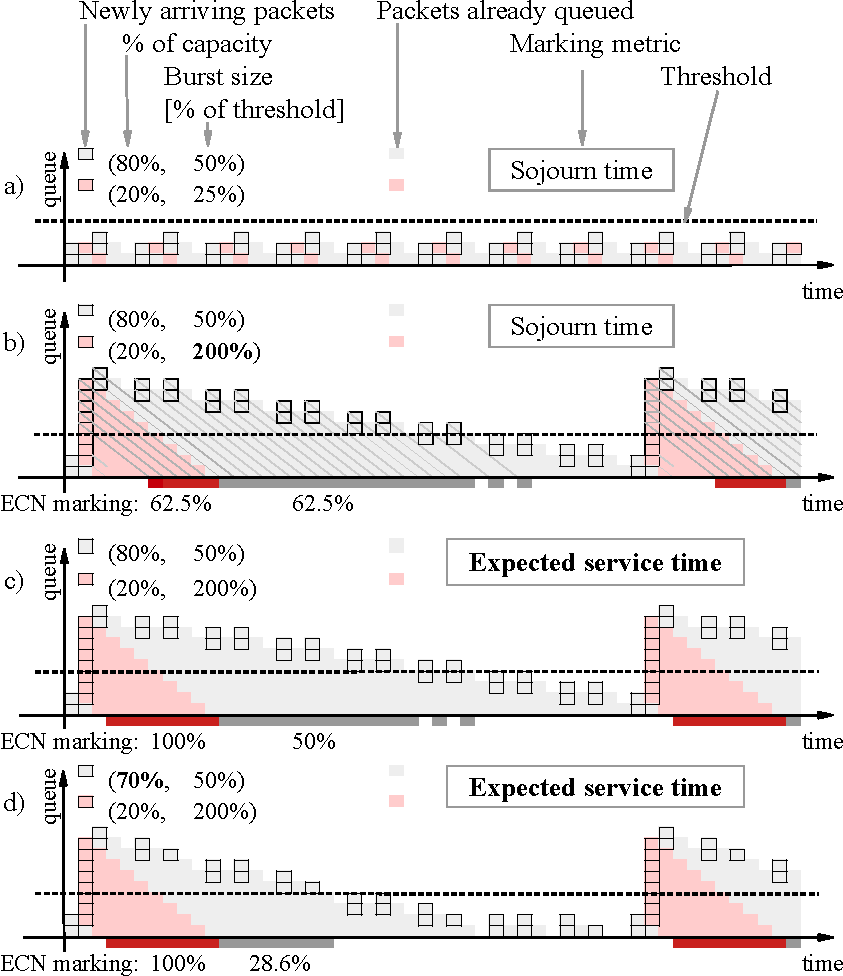
\includegraphics[width=\columnwidth]{marking-fairness}
	\caption{The Marking Fairness Problem with the Sojourn metric (b) and the ECN marking outcomes of a Solution (c--d) (see text for commentary)}\label{fig:marking-fairness}
\end{figure}

\autoref{fig:marking-fairness} shows a progression of four scenarios, reduced to their essentials by using equisized packets; one timeslot per delivered packet; a constant rate link; no congestion control; and a step ECN marking threshold. In the first three scenarios (a--c), two flows (grey and pink) fully utilize the link, consuming 80\% and 20\% each and the grey flow arrives in bursts that occupy half the queue delay threshold in the buffer. Below the progression of traffic scenarios is described, then the marking outcomes in a second pass:
\begin{enumerate}[nosep, label=\alph*)]
	\item This is the baseline case to show that the pink flow can fill the capacity left by the grey flow without exceeding the threshold, as long as it keeps its bursts small enough (in this case just 25\% of the threshold, making at most 75\% if one were to coincide with a grey burst). 
	\item In this case, each burst from the pink flow occupies 200\% of the threshold in the buffer and arrives when one packet of a grey two-packet burst is left in the queue. The average rate of both flows is unchanged, so the link is still 100\% utilized, but the grey flow still arrives in the same pattern of small bursts. So, in the time the pink burst takes to drain, some grey bursts back up behind it and, while they are draining, more small grey bursts accumulate. So the queue only finally empties just as the cycle starts to repeat.
	\item The arrivals in this scenario are identical to (b), but the marking algorithm is different (see later).
	\item In this last case, the pink flow stays unchanged at 20\% of the link and still in large bursts twice the depth of the threshold. However, the flow rate of the grey flow reduces from 80\% to 70\% of the link by halving every fourth burst. This is an attempt to represent the grey flow starting to respond to ECN marking, while the pink flow remains unresponsive.
\end{enumerate}
The ECN marking outcome of each is as follows:
\begin{enumerate}[nosep, label=\alph*)]
	\item There is no ECN marking in this baseline case (whatever the metric).
	\item The sojourn times of 5/8 of the packets at the tail of the pink burst exceed the threshold. So the sojourn-based AQM marks 62.5\% of the pink packets at dequeue. Because grey packets back up behind the pink burst, then behind themselves, their sojourn time exceeds the threshold for the first 62.5\% (5/8) of the grey packets between each pair of pink bursts. Thus, the marking probability of the two flows is equal, even though the pink flow is a lot more bursty.
	\item Here the evolution of the queue is identical to scenario (b), but marking is based on a metric we call `expected service time' rather than sojourn time. This will be fully explained in \S\,\ref{sec:exp_svc_time}, but for now it is enough to say that it marks a packet just before it is dequeued based on whether the backlog \emph{at that instant} is expected to need longer than the threshold to drain. This increases the pink marking probability from 62.5\% to 100\%. In contrast, marking shifts away from grey packets, as grey marking reduces from 62.5\% to 50\%.
	\item As the load from grey traffic falls a little, the queue falls below the threshold considerably sooner, considerably reducing the grey marking probability. Indeed a reduction of the grey traffic by 1/8 reduces grey marking probability by more than 3/8 (from 50\% to below 29\%). Nonetheless, the AQM still marks 100\% of the pink packets, because the backed up grey packets still exceed the threshold for the whole period while the pink burst is draining.
\end{enumerate}

The wider space of scenarios like this has been investigated by varying the relative shares and relative burst sizes between flows (see \S\,\ref{sec:marking_fairness_discuss}). Although the difference between the sojourn and expected service time metrics is sometimes less dramatic and sometimes more, the following intuition is generally true for all scenarios.

A smoother flow has smaller but more frequent arrival events compared to a bursty flow. So, although the bursty flow might happen to back up behind one of the smaller bursts of the smoother flow, multiple arrival events of the smoother flow will back up behind the larger burst. Therefore proportionately more of a bursty flow will be near the head of the buffer, and the packets of a smoother flow will be more likely to be occupying the tail.

Therefore, marking the head packet when there is an excessive backlog behind it is likely to lead to fairer marking than marking the head packet because it had an excessive backlog in front of it (during its sojourn through the queue). 

% ================================================================
\section{Solution: Expected Service Time}\label{sec:exp_svc_time}

Two approaches will be proposed to minimize signalling delay. Both start with the backlog measured instantaneously at dequeue, then translate it into the expected time needed to drain this backlog---thus both measure the `expected service time':
\begin{itemize}[nosep]
	\item Time-based backlog;
	\item Scaled sojourn time.
\end{itemize}

\subsection{Time-Based Backlog}\label{sec:time-based_backlog}

In this approach, as each packet is about to be dequeued from the head of the queue, the. expected service time to clear the backlog behind it is calculated as
\[\mathrm{E(svc\_time)} = \mathrm{(backlog\_deq)}\times \frac{\mathrm{avg\_serializn\_time}}{\mathrm{(avg\_pkt\_size)}},\]
or in English, the expected service time, \(t_b^*\), to clear the backlog is the backlog at dequeue, \(b\) (e.g.\ in bytes), multiplied by the recent average serialization time of each packet, \(t_s^*\) and divided by the recent average packet size (in bytes), \(s^*\).

Multiplying by the quotient on the right is the same as dividing by the average drain rate. As with averaging any rate, the quotient should be calculated as a quotient of averages, not an average of quotients. This is particularly important if the drain rate varies considerably. Also the averages should be exponentially weighted moving averages (EWMAs) with high gain, e.g. \(g=\sfrac{1}{2}\), so that they respond rapidly to changing delivery rate. The gain should be an integer power of 2 so that it can be implemented as a bit-shift.

For instance, assuming the times when dequeue of the previous packet started and ended were stored as \(t_1\) \& \(t_2\) and the packet size was \(s\), the EWMAs would be updated as
\begin{align}
	t_s^* &= g\left((t_2-t_1) - t_s^*\right)\notag\\
	s^*   &= g(s - s^*)\notag
\intertext{The expected time to clear the backlog is then,}
	t_b^* &= b * t_s^* / s^*.\label{eqn:t-based_backlog}
\end{align}
While the buffer is non-empty, the time that dequeue ends, \(t_2\) will typically become the time that serialization of the next packet starts. Reusing the same time value for both will ensure that any error introduced by coarse clock precision is averaged out. 

On the other hand, if the buffer was empty when the previous packet finished dequeuing, the time that serialization took has to be used, without including the idle time waiting for the next dequeue to start.

Note that any media acquisition delay should not be counted, and the backlog that builds while waiting to acquire the medium should not be counted for AQM marking, because it is not caused by the load from the sender, and therefore cannot be reduced by getting the sender to slow down.

\subsubsection{Rationale for Time-Based Backlog}\label{sec:time-based_backlog_justify}

The time-based backlog approach assumes that the drain rate to clear the backlog will be similar to that averaged over the last few packets. There is no reason to believe that the recent drain rate is the best estimate of the rate at which the backlog will drain. For instance, a radio link is continually testing different rates to find which is the best and if a queue is continually yielding to a higher priority queue, it will proceed in fits and starts. However, for the purpose of signalling congestion, the recent drain rate gives the best available estimate of the time to drain the backlog, which itself was a result of the recent drain rate.

It should be pointed out that sojourn time also measures the drain rate over the last few packets. But it is indisputable that it is better to use a recent drain rate to estimate how fast the current backlog will drain, rather than just measuring how long it took an earlier backlog to drain that happened to be in front of the head packet when it arrived---while ignoring the current backlog.

One might consider estimating the recent drain rate from the size of just the single most recent head packet and the time to dequeue it. However, such an approach is prone to errors due to coarse clock precision or interruptions affecting access to the clock. By using EWMAs, any such errors should average out, while using a high gain keeps the measurement lag down to about two packets.

The time-based backlog approach is similar to that used in PIE, except with PIE the backlog is divided by the average drain rate over sixteen contiguous packets, and whenever the queue is not that long, the last available average rate is used.

\subsubsection{Size-Adjusted Threshold(s)}\label{sec:time-adj_thresh}

The following technique is really just an optimization of the time-based backlog. It avoids the per-packet division in \autoref{eqn:t-based_backlog} above.

It is easiest to explain with an example AQM algorithm. Say, for instance that the AQM marks packets if queuing delay exceeds a simple step threshold, \(T\). Then, as each packet is dequeued, instead of comparing the time-based backlog with the threshold queuing delay, the AQM marks a packet if
\begin{equation}
	b * t_s^* \ge s^* * T.
\end{equation}
In other words, instead of using the average packet size to scale down the backlog, it is used to scale up the threshold.

A similar approach would be used for other AQM functions. For instance, if the likelihood of marking increases by a linear ramp function, both the min and max thresholds of the ramp would be scaled up by \(s^*\).

An alternative optimization would be to ammortize the per packet calculation over a certain number of packets by accumulating the combined dequeue times of a certain number of packets and accumulating the sum of their sizes. Then every so often updating the two EWMAs, and calculating \(s^* * T / t_s^*\) to give a new threshold in bytes to compare the backlog against. However, the per-packet processing cost of the original size-adjustment is already fairly minimal (two adds, a bit-shift and two integer-multiplies).

\subsection{Scaled Sojourn Time}\label{sec:scaled_svc_time}

Another approach would be to scale the sojourn time by the ratio of the backlogs at dequeue and enqueue. That is, the expected service time at any instant would be:
\[\mathrm{E(svc\_time)} = \mathrm{sojourn\_time} \times \frac{\mathrm{backlog\_deq}}{\mathrm{backlog\_enq}},\]
where \(\mathrm{backlog\_enq}\) can be written into the packet's metadata at enqueue, along with the arrival time, which is how sojourn time is already implemented.

\subsubsection{Rationale for Scaling Sojourn Time}\label{sec:inst_svc_time_justify}

Scaled sojourn time is comparable to the above `time-based backlog' approach, but with the drain rate measured over the sojourn time of each head packet, which is equivalent to \(\mathrm{backlog\_enq}/\mathrm{sojourn\_time}\). There are two disadvantages, but one advantage, to measuring over a sojourn time.
\begin{description}
	\item[Disadvantage 1:] The measurement delay depends on the queuing delay, which makes it problematic to signal bursts quickly;
	\item[Disadvantage 2:] Each sojourn measurement is sensitive to errors reading the clock and, when the ratio of the backlogs is large, as it is during a burst, any error will be greatly magnified;
	\item[Advantage 1:] Like sojourn time, scaled sojourn time can be measured over an arbitrarily complex set of queues, by only measuring the time of first enqueue and last dequeue and the backlog at enqueue and dequeue times.
\end{description}

Scaled sojourn time would not normally be of interest because of the two disadvantages. However, where an existing deployment or a complex queue structure makes the other approaches infeasible, the advantage of scaled sojourn time might outweigh these disadvantages (but see \S\,\ref{sec:sojourn-distrib}).

Scaling the sojourn time might also make more sense if an implementation is already measuring the sojourn time for another reason. Then it will not need any additional measurement code, because it might already need to maintain the backlogs to do basic queue handling.

\begin{figure}[h]
	\centering
	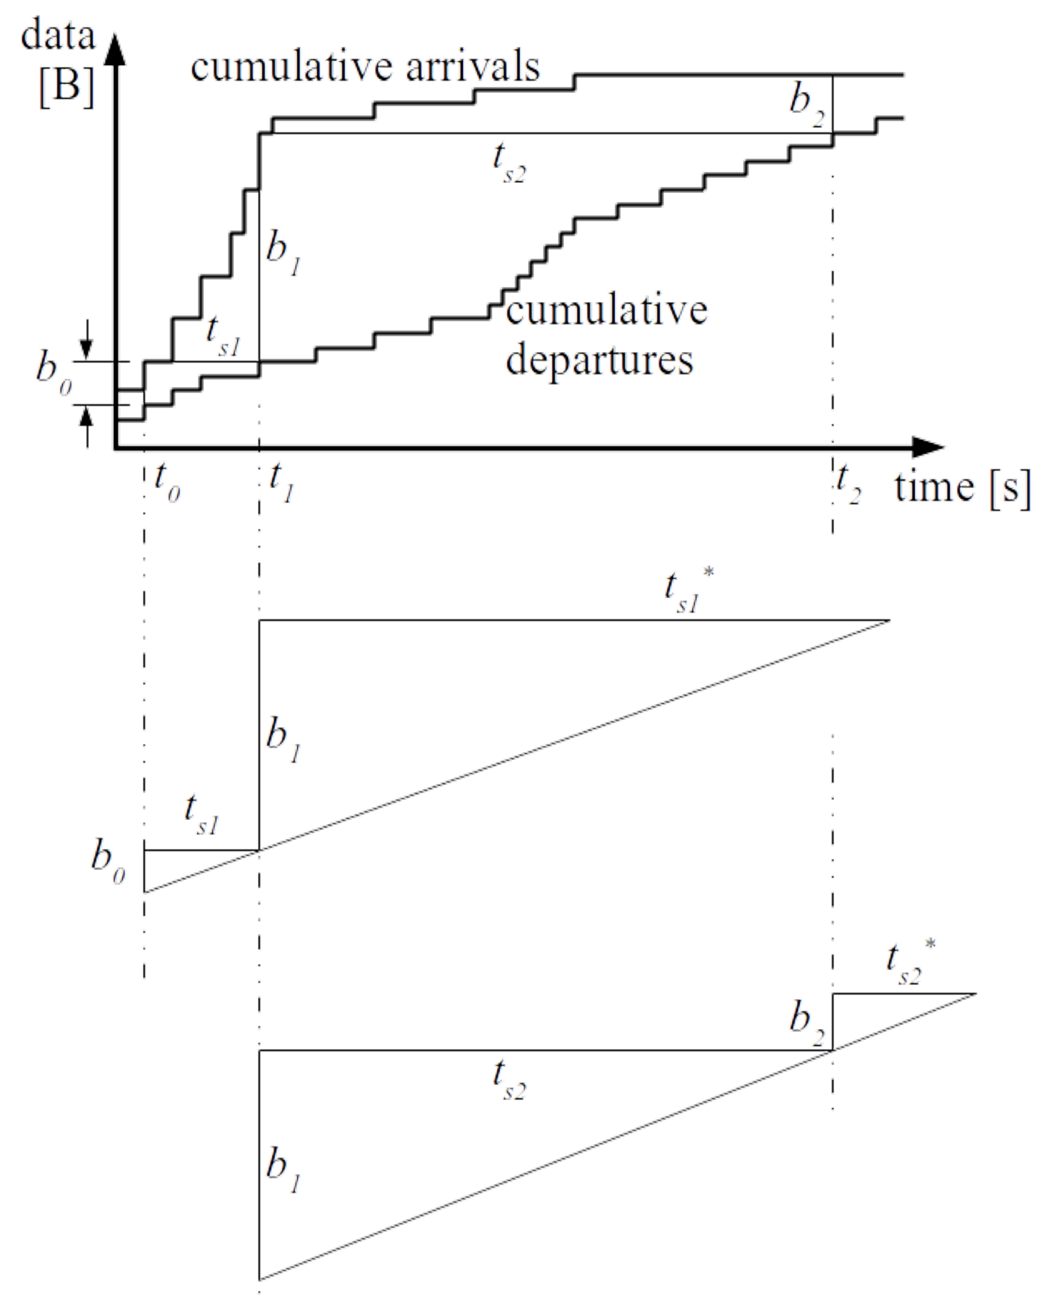
\includegraphics[width=\columnwidth]{scaled-sojourn}
	\caption{Rationale for Scaling Sojourn Time}\label{fig:scaled-sojourn}
\end{figure}

\autoref{fig:scaled-sojourn} visualizes a geometric interpretation of the rationale for scaling the sojourn time. The two plots in the chart at the top of the figure show cumulative arrivals and departures of data in packets. Between times \(t_0\) and \(t_1\) a burst of packets arrives and between \(t_1\) and \(t_2\) a few packets arrive at first, then none. Over the whole time the departure rate is varying independently as, for example, a radio link would. At any time, for instance \(t_1\), the sojourn time  (\(t_{s1}\)) can be visualized as the horizontal distance back from the departures plot to the arrivals plot. And the backlog is shown as the vertical distance between the plots (\(b_1\)).

It can be seen that the sojourn time (\(t_{s1}\)) between \(t_0\) and \(t_1\) takes account of the departure rate, but not the arrival rate (the burst), during that time. It is proposed to scale the sojourn time by the ratio of the backlogs at departure and arrival of the packet. That is \(t_{s1}^* = t_{s1} b_1/b_0\). This scaled sojourn time uses all the latest information available at time \(t_1\). 

The schematic in the middle of the figure shows, using similar triangles, how scaled sojourn time is constructed.  The departure rate during the sojourn is represented by the slope of the smaller of the middle triangle. The larger triangle extrapolates that departure rate to predict the time (\(t_{s1}^*\)) that it will take for the most recent backlog to drain.

The lower schematic shows the situation at time \(t_2\). The actual sojourn time of the new head packet \(t_{s2}\) is slightly shorter than the prediction \(t_{s1}^*\). From this new actual sojourn time, a new prediction can now be constructed  from the slightly steeper rate slope. This time the backlog \(b_2\) has reduced  during the sojourn of the head packet, because there has been a lull in arrivals since \(t_1\). Therefore the formula predicts that the sojourn time will be scaled down relative to its measured value.

We will now return to time \(t_1\) and derive the scaled sojourn time algebraically, rather than geometrically. The departure rate during the sojourn of the head packet is
\begin{align}
	r_{d1} &= \frac{b_0}{t_{s1}}.\label{eqn:drate}
\intertext{The expected service time to drain the backlog at \(t_1\) is}
	t_{s1}^* &= \frac{b_1}{r_{d1}}.\notag
\intertext{Substituting from \autoref{eqn:drate}:}
				&= t_{s1} \frac{b_1}{b_0}.\label{eqn:sojourn}
\end{align}

The expected service time can also be expressed in terms of a ratio of average arrival and departure rates during the sojourn, \(r_{a1}\) and \(r_{d1}\). The backlog at \(t_1\) can be expressed in terms of the arrival rate over the sojourn time:
\begin{align}
	b_1 &= t_{s1} r_{a1}.\label{eqn:backlog}
\intertext{Substituting this into \autoref{eqn:sojourn}, the scaled sojourn time at \(t_1\),}
	t_{s1}^* &= t_{s1} \frac{r_{a1}}{r_{d1}}
\end{align}
That is, scaling the sojourn time by the ratio between the backlogs at dequeue and enqueue is equivalent to scaling it by the ratio between the average arrival and departure rates between enqueue and dequeue.

\subsubsection{Implementing Scaled Sojourn Time}\label{sec:inst_svc_time_impl}

To implement scaling of the sojourn time, it is probably easiest to store \texttt{backlog\_enq} in the packet's metadata when the packet is enqueued. Then at dequeue it can be divided into \texttt{backlog\_deq}. 

But some implementations choose not to do too much at dequeue, because there is limited time between the packet reaching the head of the queue and starting to be forwarded. Therefore, it could be challenging to measure the system time, subtract the stored timestamp then also scale the result by a ratio.

The division in the ratio can be avoided by in at least two ways:
\begin{itemize}[nosep]
	\item Multiply the threshold(s) of the AQM by \texttt{backlog\_enq} rather than dividing it into \texttt{backlog\_deq} (as in \S\,\ref{sec:time-adj_thresh});
	\item Use the techniques below to optimize execution, although efficiency will be machine-architecture-dependent, and precision is only to the nearest binary order of magnitude:
\end{itemize}

{\small\texttt{qdelay <<= (lg(backlog\_deq) - lg(backlog\_enq)\\+ 1/2)}}\\
It is roughly equivalent to multiplying by the ratio between the backlogs, to the nearest integer power of 2.

The \texttt{<<=} operator bit-shifts \texttt{qdelay} to the left by the expression on the right. \texttt{lg()} is the logarithm function base 2. The expression bit-shifts \texttt{qdelay} to the left by the difference between the logs of the backlogs at enqueue and dequeue. The addition of 1/2 is necessary so that integer truncation of the result will round to the nearest integer, rather than always rounding down. 

The \texttt{clz()} function to count leading zeros could be used as a cheaper but more approximate base-2 log function, as follows:\\
{\small\texttt{qdelay <<= (clz(backlog\_enq) - clz(backlog\_deq))}}\\
This also avoids the need for any boundary checking code.

For example, if the \texttt{backlog\_*} variables are 32-bit unsigned integers and
\begin{itemize}[nosep]
	\item[] \texttt{backlog\_enq = 3000}, so \texttt{clz(3000)=20}
	\item[] \texttt{backlog\_deq = 30000}, so \texttt{clz(30000)=17}
\end{itemize}
Then
\begin{itemize}[nosep]
	\item[] \texttt{qdelay <<= 20 - 17}
\end{itemize}
is the same as
\begin{itemize}[nosep]
    \item[] \texttt{qdelay *= 2\^{}3},\\
\end{itemize}
which scales qdelay by 8, which approximates to \texttt{30,000/3,000 = 10} but is an integer power of 2. This is sufficient to scale the sojourn time to the correct binary order of magnitude, while still taking account of all the latest information in the queue.

However, \texttt{clz()} introduces truncation bias because it always rounds down, which could lead the result to be persistently out by up to \(\times2\) or \(/2\) for a particular target sojourn time. Using the \texttt{lg()}-based expression could be out by from \(\sqrt{2}\) to \(1/\sqrt{2}\), but with no bias---it is equally likely to be out either way.

A high performance implementation will maintain the backlog of a queue by maintaining two variables (much like the two plots at the top of \autoref{fig:scaled-sojourn}):
\begin{itemize}[nosep]
	\item[] \texttt{count\_enq} written solely by the enqueue routine;
	\item[] \texttt{count\_deq} written solely by the dequeue routine
\end{itemize}	
Then the backlog can be measured as \texttt{count\_enq - count\_deq}. These two shared variables can be read from any routine, but they are only incremented by the routine that owns them, which avoids the performance hit of a mutual exclusion lock. The two counters monotonically increase like the system clock for the sojourn measurement, but at the rate of data transfer in and out respectively, not the rate of time passing. 

\subsection{Distributed Queues}\label{sec:sojourn-distrib}

Using sojourn time leverages the advantage that it can be measured across a complex set of queues, including the case where the initial enqueue and the final dequeue routines are distributed across different machines or processors, as already mentioned (separate clocks would need to be synchronized).

This could include the case where the inputs are located on multiple client machines (e.g.\ mobile user equipment, WiFi stations, cable modems or passive optical network modems) while the output is a located at an aggregation node (e.g.\ a cellular base station (eNodeB)~\cite{Tan09:AQM_uplink_patent}, a WiFi access point (AP), a centralized controller for multiple WiFi APs, a cable modem terminal server (CMTS) or optical line termination (OLT) equipment), with a multiplexed access network between the clients and the aggregation node.

In complex cases like these, if minimization of measurement delay is important, the best approach to use will depend on which of metrics are most feasible to measure and communicate to the dequeue process, which will depend on the architecture of the distributed queues. \autoref{tab:distrib-qs} tabulates which metrics are needed by which approach.

\begin{table*}[h]
	\begin{center}
		\begin{tabular}{ll|cc}
						& 				& Time-based backlog & Scaled sojourn time\\
			\hline
			\multirow{2}{*}%
			{enqueue time}& arrival time	& -					& \checkmark \\
						& backlog		& -					& \checkmark \\
			\hline
			\multirow{4}{*}%
			{dequeue time}& departure time& \checkmark		& \checkmark \\
						& backlog		& \checkmark		& \checkmark \\
						& serial'n time	& \checkmark		& - \\
						& packet size	& \checkmark		& - \\
		\end{tabular}
	\end{center}
	\caption{Metrics needed by each approach}%
	\label{tab:distrib-qs}
\end{table*}

Note that the backlog at enqueue time and the backlog at dequeue time need to include all the data buffered between the two, not just that in the ingress and egress buffers. Therefore the backlog metric is probably the critical factor for feasibility. And given both approaches need the backlog at dequeue time, and scaled sojourn also needs the backlog at enqueue time, scaled sojourn might end up being the more complex approach.`

For instance, on a single machine, the \texttt{count\_enq} variable would be available in a memory shared between ingress and egress. But if the ingress and egress are separate, the ingress machine would have to communicate the \texttt{count\_enq} variable to the egress over a (preferably non-blocking) control channel, so that the egress could calculate \texttt{backlog\_deq} by subtracting \texttt{count\_deq}. 

Certain access network technologies, e.g.\ those for cellular radio access networks, already include such a control channel, over which buffer status report (BSR) control messages are sent from the user equipment at the ingress to the radio network controller. The delay to access a control variable at the input machine from the output machine would be larger than that in a non-distributed system, but it would at least be a known, constant delay. So the control system could still provide robust metrics to control queuing in the data channel.

As well as the aggregation node using expected service time to apply congestion signalling within the final dequeue routine (effectively on behalf of the input queue), the aggregation node could also use expected service time to govern the scheduling algorithm for controlling each client's inward (upstream) access rate into the shared medium, by altering the rate at which it granted medium access slots to each client.

\subsection{Applicability of Expected Service Time}\label{sec:inst_svc_time_applic}

Using any of the approaches in \S\,\ref{sec:exp_svc_time} to calculate expected service time would improve timeliness relative to using sojourn time or other techniques to measure queue delay. However, it would not be worth modifying an existing deployment unless all other delays were going to be removed at the same time. 

It might be thought that an algorithm like the proportional integral (PI) controller\footnote{Used in QCN~\cite{IEEE802.1Qau:Ethernet_QCN}, PIE~\cite{Pan17:PIE}, PI2~\cite{DeSchepper16a:PI2} or the base AQM of DualPI2~\cite{Briscoe15e:DualQ-Coupled-AQM_ID}.} already takes account of the change in queuing delay between samples, so changing the queuing delay measurement itself seems redundant. However, using expected service time actually ensures that a PI algorithm takes account of the change between the latest queue delay measurements at each sample time, not between two outdated measurements.

It might also be thought that PI controllers do not need to care so much about instantaneous measurements, because they are maintaining the fairly large queue that is needed by classic TCP algorithms like Reno, Cubic, Compound or BBR. However, even though a PI algorithm only samples the queue fairly infrequently (relative to packet serialization time), using an out of date queue metric makes it necessary to introduce extra heuristic code to deal with the resulting sloppiness.

For instance, in the case of PIE~\cite{Pan17:PIE}, some heuristic code suppresses any drop once the last sample of queue delay falls below half the target delay.\footnote{As long as some other conditions hold that are not important here.} This is an attempt to suppress drop when the queue is draining after the load has gone idle. However, it is ineffective if sojourn time is used to measure the queue, because the sojourn time does not reduce until after the last packet (as explained on the right of \autoref{sojourn-prob}). Using expected service time whenever it is sampled should eliminate the need for this heuristic because it takes account of the reducing backlog as the queue drains.\footnote{Indeed, this was the original motivation for this work.}

Expected service time is also applicable to the CoDel algorithm for the same reasons---sojourn time fails to take account of the evolution of the queue after the head packet was enqueued (again, as in \autoref{sojourn-prob}). This can tend to cause the AQM to continue dropping or marking packets at the end of a flow, because the sojourn time does not recognize that the queue has gone below the target delay. The CoDel code in Linux includes a heuristic to exit dropping mode when the backlog goes below 1\,MTU, but that still continues dropping mode until the last packets of a flow, and tail loss is particularly problematic for a flow to detect.

Expected service time is particularly applicable to a simple AQM algorithm like the time-based shallow threshold recommended for DCTCP in~\cite{Bai16:MQ-ECN} or the native AQM for L4S traffic in DualPI2~\cite[Appx.\ A]{Briscoe15e:DualQ-Coupled-AQM_ID} or Low Latency DOCSIS~\cite{CableLabs:DOCSIS3.1}. It would be applicable whether the threshold is a simple step, or a probabilistic ramp like the RED function (but based on instantaneous queue delay, not smoothed queue length), or a deterministic ramp or convex function of instantaneous queueing delay, as in Curvy RED~\cite[Appx.\ B]{Briscoe15e:DualQ-Coupled-AQM_ID}. The queue in these cases is intended to be very shallow, so it might seem that the extra measurement delay would be minimal. However, the sensitivity of these very low delay schemes to burstiness makes it particularly important to ensure that bursts are measured rapidly and correctly.

Expected service time could apply to many types of queue, not just packet queues, as long as the size of each job is quantified in common units that are additive. Examples include, but are not limited to, queues of datagrams, frames or packets, as well as message queues, call-server queues, computer process scheduling queues, storage queues (e.g. SSD or disk), workflow queues for mechanical or human-operated stages of tasks. 

As well as dropping or ECN-marking, different sanctions could be applied using the same basic ideas. Examples include, but are not limited to: truncating or otherwise damaging the data or checksum of a message or packet but preserving the information necessary for delivery; rerouting; delaying; downgrading the class of service; and tagging.

% ================================================================
\section{Marking Fairness: Discussion}\label{sec:marking_fairness_discuss}

\todo{Give results of a scan of the range of marking outcomes as flow shares and relative burstiness vary}


\todo{Discuss lack of definition of marking fairness and discuss SPSP}



\todo{Subsection to discuss potential for Queue Protection without per-flow state.}

% ================================================================
\section{Other Signalling Delays}\label{sec:other_delays}

The introduction enumerated six causes of delay to congestion signals and highlighted two that this memo would focus on. The other four sources of signalling delay are briefly surveyed below, with pointers to other work where they have been considered.

\paragraph{Propagation Delay:} Numerous proposals have been made to speed up signalling by sending the signal from the queue back against the flow of traffic, direct to the sender. This can be done in a pure L2 network, e.g. backwards congestion notification (BCN) in IEEE 802.1Qau~\cite{IEEE802.1Qau:Ethernet_QCN} a.k.a.\ Quantized Congestion Notification (QCN), which is now rolled into 802.1Q-2011 and 802.1Q-2014. However, in general signalling backwards is problematic in IP networks, amongst other reasons because the sender has to accept out-of-band packets from any arbitrary source in the middle of the network, which makes it vulnerable to DoS attacks~\cite{IETF_RFC6633:ICMP_SQ_Depr}. 

Therefore, here we will assume that signals are piggy-backed on the forward traffic flow then fed back to the sender via the receiver. However, this does not preclude a solution to the problems of backwards congestion notification.

\paragraph{Smoothing Delay:} AQMs designed for the Internet's classic congestion controls (TCP Reno, Cubic, Compound, etc.) filter out fluctuations in the queue by smoothing it before using the smoothed measurement as a measure of load to drive the congestion signal. DCTCP proposed to smooth the signal at the sender, so that the network could send out the signal immediately, without smoothing, and L4S followed this approach~~\cite{Briscoe16a:l4s-arch_ID}. This allows the sender to receive the signal without smoothing delay, which is particularly useful in cases where the sender might not need to smooth the signal itself, e.g.\ to detect overshoot when accelerating to start a new flow. Shifting the smoothing function from the network to the sender also makes sense because the network does not know the round trip time (RTT) of each flow, so it has to smooth over the maximum likely RTT. Whereas a sender knows its own RTT and can smooth over this timescale.

\paragraph{Signal encoding delay:} Previous research has proposed to change the IP wire protocol to provide more bits to signal congestion. Nonetheless, it has been pointed out that the delay of a unary encoding is inversely proportional to the value being encoded, and the congestion window of a scalable congestion control is also inversely proportional to the value of the congestion signal. So, as flow rates (and consequently congestion windows) increase over the years, at least in general the delay to encode the signal does not increase.\footnote{However, encoding delay does increase with the degree of ACK coalescing.}

Therefore, in this report we have assumed a standard unary encoding of congestion signals. This does not preclude other encodings, e.g. the multi-bit encoding of QCN or minor alterations to the decoding to avoid saturation, such as that in \cite{Briscoe17a:CC_Tensions_TR}.

\subsection{Removing Randomness Delays}\label{sec:rand_delay}

One of the main motivations for the design of Random Early Detection (RED)~\cite{Floyd93:RED} was to introduce randomness to break up synchronization between the sawteeth of TCP flows driving the same queue. This still remains an important requirement for all AQM algorithms~\cite{Baker15:AQM_Recommendations}.

With clean-slate approaches such as DCTCP in private networks, or incrementally deployable clean-slate approaches like L4S~\cite{Briscoe16a:l4s-arch_ID} for the public Internet, requirements for the network and for end-systems are still in the process of definition. In these clean-slate or slightly dirty-slate cases, it would be possible to require the sender's congestion control to dither its response to congestion signals, so that it would not be necessary to introduce randomness in the network, which adds uncertainty and therefore delay to the congestion signalling channel. 

Any AQM that probabilistically signals congestion with probability \(p\) could deterministically signal congestion by introducing an interval of \(1/p\) packets between each drop or mark. 

The determinism would be lost wherever the AQM was controlling flows mulitplexed within one queue without per-flow state, because assignment of each deterministic congestion signal to each flow would become randomized by even slightly random packet arrivals from the different flows~\cite{Briscoe15d:PIE_rvw}.

Nonetheless, whenever a flow is on its own in an AQM, which is a common case for the traffic patterns in many access network designs,  deterministic congestion signalling would reduce signalling delay. This could particularly ease the design of new flow-start algorithms, where the flow introduces microbursts or chirps to sense at what level it starts to congest the link.

\todo{Explain the distinction between the marking algo determining when the next mark occurs and the CC sawtooth turning marking on and off.}

PDPC+~\cite{Sagfors03:PDPC_vary} and CoDel~\cite{Nichols12:CoDel}, which is very similar, use a deterministic rather the probabilistic algorithm to encode the congestion signal. However, they do not propose a way to introduce randomness in the end-systems instead. Therefore, they are likely to be prone to synchronization effects.